\documentclass[assignmentprobability_basics_Solutions]{subfiles}

\IfSubStr{\jobname}{\detokenize{Solutions}}{\toggletrue{solutions}}{\togglefalse{solutions}}

\fancypagestyle{firstpage}

{\rhead{Probability Basics \linebreak \textit{Version: \today}}}

\title{Probability Basics}
\author{A Computational Introduction to Robotics}
\date{Fall 2020}

\begin{document}

\maketitle
\thispagestyle{firstpage}


\begin{learningobjectives}
\bi
\item Define the concept of a probability.
\item Learn Bayes' rule and other rules for manipulating probabilities.
\ei
\end{learningobjectives}

\section{Motivation}

It turns out that the notion of probability provides us with a powerful method to formalize the concept of uncertainty and allows us to reason about many types of uncertainty in a unified way.  Formalizing uncertainty using probability theory will enable us to solve robotics challenges in a principled and robust manner.

\bi
\item make explicit our assumptions about the uncertainties present within our sensor data and the impact of these uncertainties on predictions based on that data.
\item allow us to quantify confidence in our predictions
\ei

\section{Probability}

Hopefully the previous section left you feeling excited to learn more about the theory that underlies these big ideas.  Next, we'll take our first steps towards learning this theory.

\subsection{Intuition}
Most of us are used to thinking that events can be probabilistic, that is we can attach some probability to whether or not they occur.  Take for example flipping a coin.  We could think of the event that the coin comes up heads as having probability 0.5.  That is, there is an even chance that it happens versus doesn’t happen.  Further, we can say that an event is \emph{observable} if we are able to directly observe whether it occurred.  For instance, whether a coin comes up heads is an observable event since you can ultimately observe the outcome of the flip.  In contrast, some events would be considered unobservable if they are unable to be directly ascertained by human senses.  A classic example of this would be whether a scientific theory is true or not.  It is impossible to directly observe whether the theory is true, but you might be able to observe events that are consistent or inconsistent with the theory.

\vspace{1em}
\begin{exercise}[(10 minutes)]
Come up with 3ish examples of observable events that are probabilistic in nature.  For each event, provide the probability that it occurs or explain what factors would determine the probability.  Some potential ideas to get you going: sporting events, elections, weather, etc.

\begin{boxedsolution}
Here are some possible ideas.
\bi
\item The event \emph{The Nationals win the 2019 MLB World Series} is an observable event (we will ultimately find out whether or not this happens).  The probability of this event will depend on the quality of their opponent (currently this is either the Yankees or the Astros, both of whom would be favored in the series) and other factors (such as home field advantage).
\item The event the movie Joker wins the Academy Award for Best Pictures is an observable event.  The probability that it occurs will depend on the amount of money spent promoting it to academy members, the quality of other movies that are released, etc.
\ei
\end{boxedsolution}

\end{exercise}

\subsection{Formal Definition}

Next, we'll define more formally\sidenote{this is not the full definition of a \href{https://en.wikipedia.org/wiki/Probability_space}{probability space} used in modern mathematics.  For the purposes of most people that \emph{use} probability theory on actual problems, the full definition is needlessly complex.  For instance, as a grad student I (Paul) never saw the full definition in any of my ML courses.  Use the following link if you want a more \href{https://m.tau.ac.il/~tsirel/dump/Static/knowino.org/wiki/Probability_space.html}{in-depth discussion of the parts of the formal definition that are tricky} (our expectation is that you won't want this discussion!).} what we mean by a probability.  Having this formal definition will give us the ability to determine useful rules for manipulating and reasoning about probabilities.  To define the concept of a probability, we'll need to specify two ingredients.
\subsection{Events}

An \emph{event} is something that may or may not occur in response to some random process.  For instance, we could define the event that a coin comes up heads when it is flipped.  We often use capital letters to indicate events.  Since we've been using capital letters to also represent matrices, in our materials we'll use a cool mathy-looking calligraphic font to represent events.  For instance, we might use the symbol $\mathcal{H}$ to refer to the event that a coin flip comes up heads. It's important to emphasize that a single random process can have many associated events.   For instance, for the coin flip example we might also define $\mathcal{T}$ to be the event that the coin comes up tails (or $\mathcal{U}$ to indicate that event that the coin rotated at least 10 times in the air when we flipped it).

Further, events don't necessarily have to be mutually exclusive.  For instance, we might define the event $\mathcal{R}_h$ to indicate the event that the Republican party controls the majority in the House of Representatives following the 2020 election and $\mathcal{D}_s$ to indicate the event that the Democratic party controls the majority in the Senate following the 2020 election.  Both (or none) of these events could occur.

\subsection{Probability Measure Function}
The probability measure function assigns a probability to the occurrence of any particular event.  We can think of this probability measure function as taking as input an event and outputting a probability.  For instance, $p(\mathcal{E})$ provides the probability that event $\mathcal{E}$ occurs according to probability measure $p$.  All probability measure functions must satisfy the following properties.

\bi
\item $0 \leq p(\mathcal{E}) \leq 1$: the probability of an event ranges from 0 (an impossible event) to 1 (an event that will always occur).
\item Given a set of $n$ events $\mathcal{E}_1, \mathcal{E}_2, \ldots, \mathcal{E}_n$ that are disjoint (i.e., no two can occur simultaneously)
\begin{align}
p(\mathcal{E}_1~\mbox{or}~\mathcal{E}_2~\mbox{or}~\ldots~\mbox{or}~\mathcal{E}_n) = \sum_{i=1}^n p(\mathcal{E}_i) \label{eq:probunion} \enspace .
\end{align}


The equation above specifies what is sometimes called the union rule of probability.  It states that the probability of one of these disjoint events occurring must be equal to the sum of the probability of each of the events occurring.  You will also sometimes see Equation~\ref{eq:probunion} written as

\begin{align}
p(\mathcal{E}_1 \cup \mathcal{E}_2 \cup \ldots \cup \mathcal{E}_n) = \sum_{i=1}^n p(\mathcal{E}_i) \enspace .
\end{align}

If you're not familiar with the symbol $\cup$ it is the symbol for a union of two sets.  The reason you'll sometimes see this notation is that in the full definition of a probability space an event is defined as a set (as stated in the margin note earlier in this section, you need not worry about the most rigorous definition in this course).

\item Given a set of (not necessarily disjoint) events $\mathcal{E}_1, \mathcal{E}_2, \ldots, \mathcal{E}_n$ where at least one of these $n$ events must occur
\begin{align}
p(\mathcal{E}_1~\mbox{or}~\mathcal{E}_2~\mbox{or}~\ldots~\mbox{or}~\mathcal{E}_n) = 1 \enspace .
\end{align}
\ei

This rule just states that if we have an exhaustive set of events (that cover all possible cases), at least one of them \emph{must} occur.

\subsection{Complement Rule for Probability}

Given the definition of probability detailed above, it follows that if the probability of an event happening is $p(\mathcal{E})$ then the probability of the event \emph{NOT} happening is $1-p(\mathcal{E})$.   The following are common ways of to express this relationship (we'll use Equation~\ref{eq:complement} in this class).  These all say the same thing (the only difference is notation).

\begin{align}
p(\neg \mathcal{E}) &= 1 - p(\mathcal{E}) \label{eq:complement} \\
p(\mbox{not}~\mathcal{E}) &= 1 - p(\mathcal{E}) \nonumber \\
p(\overline{\mathcal{E}}) &= 1 - p(\mathcal{E}) \nonumber \\
p(\mathcal{E}') &= 1 - p(\mathcal{E}) \nonumber \\
p(\mathcal{E}^c) &= 1 - p(\mathcal{E}) \nonumber
\end{align}

We point out these alternate notations not to confuse you (we'd never do that!) but to help you interpret various external resources you might find on these topics.

\vspace{1em}
\begin{exercise}[(10 minutes)]
Here are some diagnostic questions to make sure that you got the basic ideas. 
\bes
\item Suppose $\mathcal{E}_1, \mathcal{E}_2, \mathcal{E}_3$ are disjoint events.  Further, suppose that one of these events must occur.  Which of the following functions are valid probability measure functions?

\begin{align}
p_1(\mathcal{E}_1)=\frac{1}{10} , p_1(\mathcal{E}_2)=\frac{1}{5}, p_1(\mathcal{E}_3)=\frac{7}{10} \nonumber
\end{align}


\begin{align}
p_2(\mathcal{E}_1)=\frac{11}{10} , p_2(\mathcal{E}_2)=\frac{-1}{10}, p_2(\mathcal{E}_3)= 0 \nonumber
\end{align}



\begin{align}
p_3(\mathcal{E}_1)=\frac{1}{10} , p_3(\mathcal{E}_2)=\frac{1}{5}, p_3(\mathcal{E}_3)=\frac{1}{2} \nonumber
\end{align}



\begin{align}
p_4(\mathcal{E}_1)=1 , p_4(\mathcal{E}_2)=0, p_4(\mathcal{E}_3)=0 \nonumber
\end{align}

\begin{boxedsolution}
$p_1$ is a valid probability measure function since the probabilities add up to 1 and all are non-negative.  $p_2$ is not a valid probability measure function since two of the probabilities are outside of the appropriate range $[0,1]$.  $p_3$ is not a valid probability measure function since the probabilities of the three events add up to less than 1. $p_4$ is a valid probability measure function since the probabilities add to 1 and are in the appropriate range.
\end{boxedsolution}

\item The Birthday Problem is a well-known probability problem often used in discrete math courses.  According to \href{https://en.wikipedia.org/wiki/Birthday_problem}{the Wikipedia article on the Birthday Problem}, the probability that at least two students among the 70 students in machine learning this semester share the same birthday is $0.999$.  What is the probability that no two students share the same birthday?

\begin{boxedsolution}
Notice that the event \emph{no two students share a birthday} only happens when the event \emph{at least two students share a birthday} does not happen.  Therefore, these events are complements.

\begin{align}
p(\mbox{no two students share a birthday}) &= 1 - p( \neg \mbox{no two students share a birthday})  \nonumber\\
&= 1 - p(\mbox{at least two students share a birthday}) \nonumber \\
&= 1 - 0.999  \nonumber\\
&= 0.001  \nonumber
\end{align}
\end{boxedsolution}

\ees
\end{exercise}

\section{Bayes' Rule}

\begin{externalresources}[(60 minutes)]
\begin{learningobjectives}
Note that these learning objectives have been written to be very specific (based on feedback from the course survey).  When you first read them, you probably won't know what they mean in detail.  As you go through the readings, hopefully the more precise statement of these learning objectives will be useful for assessing your understanding of the provided resources.

\bi
\item When Bayes' rule is useful (i.e., when $p(A|B)$ is easier to work with than $p(B|A)$).
\item The idea of a conjoint probability $p(\mathcal{A}, \mathcal{B})$ (note: alternate notations include $p(\mathcal{A}~\mbox{and}~\mathcal{B})$ and $p(\mathcal{A} \cap \mathcal{B})$).
\item The definition of a conditional probability $p(\mathcal{A} | \mathcal{B}) = \frac{p(\mathcal{A},\mathcal{B})}{p(\mathcal{B})}$.
\item The equation for the product rule $p(\mathcal{A}, \mathcal{B}) = p(\mathcal{B}) p(\mathcal{A} | \mathcal{B}) =  p(\mathcal{A}) p(\mathcal{B} | \mathcal{A})$ (Allen calls this the probability of a conjunction).
\item The equation for Bayes' rule $p(\mathcal{A} | \mathcal{B}) = \frac{p(\mathcal{B} | \mathcal{A}) p(\mathcal{A})}{p(\mathcal{B})}$.
\ei
\end{learningobjectives}

Allen Downey (ever heard of him?) wrote an excellent book called Think Bayes that introduces Bayesian analysis.  The \href{http://www.greenteapress.com/thinkbayes/html/thinkbayes002.html}{first chapter} (which you should read) starts with a less formal definition of probability than the one we gave earlier.  The chapter then gives intuitions around conjoint probability (the probability that multiple events occur simultaneously), conditional probability (the probability that some event occurs conditioned on another event having occurred), and finally to Bayes' rule (a surprisingly easy theorem to derive that allows you to write one conditional probability distribution in terms of another).  The Monty Hall problem in section 1.7 is probably okay to skim (see Allen's note at the end of that section for why this is the case).

Allen's treatment of the material is, of course, not the only one out there (we like it for its focus on building intuition and focusing on the key ideas).  Here are some other resources you might consider checking out (they are optional).
\bi
\item \href{https://www.khanacademy.org/partner-content/wi-phi/wiphi-critical-thinking/wiphi-fundamentals/v/bayes-theorem}{Khan Academy Video on Bayes' Theorem} shows some simple applications of Bayes' rule and explains why it is a convenient way to reason about the probability of hypothesis given data).
\item \href{https://www.youtube.com/watch?v=R13BD8qKeTg}{Veritasium Episode on Bayes' Theorem} has a bit more history and philosophy of Bayes' Theorem along with some nice visualizations.  It also includes the presenter walking on a very scenic mountain (for some reason), so there's that if nothing else.
\item Julia Galef's video \href{https://www.youtube.com/watch?v=BrK7X_XlGB8}{A Visual Guide to Bayesian Thinking}
\item I (Paul) ran across \href{https://youtube.com/watch?v=nvqXXlz-rx0}{this example of applying Bayes' rule to a real world problem}.  It was created by a grad school friend of mine and is hilarious (lots of Cat Memes).  I did notice that there is a mistake in the math at the 8:12 mark in the video (he states that $p(\mbox{alarm} | \mbox{no theft}) = 1 - p(\mbox{alarm} | \mbox{theft})$, which is not necessarily the case).  It's still a good video though.
\ei

\end{externalresources}

\begin{exercise}[(20 minutes)]
\begin{notice}
If you are having trouble dealing with the denominator that you get when you apply Bayes' rule, you may want to skip ahead to the section on the \emph{Marginalization Rule for Probabilities} and then return to these problems.
\end{notice}
\bes
\item You are given three coins.  Two are of type 1, we'll call this type $\mathcal{C}_1$, and one is of type 2, we'll call this type $\mathcal{C}_2$. If you flip a coin of type 1, the coin will come up heads with probability $\frac{4}{5}$ (i.e., $p(\mathcal{H} | \mathcal{C}_1) = \frac{4}{5}$). If you flip a coin of type 2, the coin will come up heads with probability $\frac{1}{2}$ (i.e., $p(\mathcal{H} | \mathcal{C}_2) = \frac{1}{2}$).  Suppose you choose one of the three coins (there is no way for you to tell them apart), flip it once, and it comes up heads.  What is the probability that you flipped a coin of type 2 (i.e., what is $p(\mathcal{C}_2 | \mathcal{H})$)?  After you compute your answer, compare it with the probability that a randomly selected coin was of type 2 (before you flipped it and observed heads).  Does the relationship between this prior probability and the posterior probability make sense?

\begin{boxedsolution}
\begin{align}
p(\mathcal{C}_2 | \mathcal{H}) &= \frac{p(\mathcal{H} | \mathcal{C}_2) p(\mathcal{C}_2)}{p(\mathcal{H})} & \mbox{Bayes' Rule} \nonumber \\
&=  \frac{p(\mathcal{H} | \mathcal{C}_2) p(\mathcal{C}_2)}{p(\mathcal{C}_1) p(\mathcal{H}|\mathcal{C}_1) + p(\mathcal{C}_2) p(\mathcal{H}|\mathcal{C}_2)} & \mbox{expand denominator} \nonumber \\
&= \frac{ \frac{1}{2} \times \frac{1}{3}}{\frac{4}{5} \times \frac{2}{3} + \frac{1}{2} \times \frac{1}{3}} &\mbox{plug in numbers} \nonumber \\
&= 0.238 \nonumber
\end{align}

The posterior probability ($0.238$) we computed is less than the prior probability ($\frac{1}{3}$).  This makes sense since a heads is more probable if we have a coin of type 1, so observing a heads should push our beliefs towards the coin being of type 1.
\end{boxedsolution}


\item You train a neural network to identify whether \href{https://www.freecodecamp.org/news/chihuahua-or-muffin-my-search-for-the-best-computer-vision-api-cbda4d6b425d/}{an image contains a picture of a Chihuahua or a Blueberry Muffin} (you know you want to click the link!).  Let's further assume that there are no images that contain both a muffin and a Chihuahua (of course as we all know Chihuahuas love muffins).  Based on your project report for module 1, you know that if the image contains a Chihuahua, your model will identify it as such with probability 0.9.  Also, you know that if the model contains a muffin, your model will identify it as such with probability 0.8.  You now decide to test your model on a dataset which contains 80\% muffins.  Assuming that your model predicted that an image contained a muffin, what is the probability that it actually contains a muffin? (you can assume that the performance of your model doesn't change when run on this new dataset).

\begin{boxedsolution}
Let $\mathcal{M}$ represent the event that the image contains a Muffin.  Let $\mathcal{D}_M$ represent that a muffin was detected in the image.
\begin{align}
p(\mathcal{M} | \mathcal{D}_M) &= \frac{p(\mathcal{D}_m | \mathcal{M})  p(\mathcal{M})}{p(\mathcal{D}_M)} \\
&= \frac{p(\mathcal{D}_m | \mathcal{M})  p(\mathcal{M})}{ p(\mathcal{D}_m | \mathcal{M})  p(\mathcal{M}) + p(\mathcal{D}_m | \neg \mathcal{M})  p(\neg \mathcal{M})} \\
&= \frac{0.8 \times 0.8}{0.8 \times 0.8 + 0.1 \times 0.2} \\
&= 0.97
\end{align}
\end{boxedsolution}
\ees
\end{exercise}

\section{Marginalization Rule for Probabilities}
The application of Bayes' rule often proceeded according to the following outline.  First, we would define an event we want to reason about. For instance, we might define $\mathcal{D}$ as the event that a person has a disease and $\mathcal{S}$ as the event that a particular symptom is observed.  If we want to know $p(\mathcal{D} | \mathcal{S})$ we apply Bayes' rule like so.

\begin{align}
p(\mathcal{D} | \mathcal{S}) &= \frac{p(\mathcal{S} | \mathcal{D}) p(\mathcal{D})}{p(\mathcal{S})}
\end{align}

In order to calculate $p(\mathcal{S})$, some of the resources simply gave a number (e.g., in the Khan Academy video the premise was that you Googled to find this value), used a convenient trick to get it (as in Allen's M\&M example), or used the following calculation (as in the Veritasium and the Car Alarm videos).

\begin{align}
p(\mathcal{S}) &= p(\mathcal{D}) p(\mathcal{S}|\mathcal{D}) + p(\neg \mathcal{D}) p(\mathcal{S} | \neg \mathcal{D}) \label{eq:bayesdenominator}
\end{align}

We wanted to revisit this calculation as it is hiding away some pretty powerful and interesting stuff.  This calculation can be derived using the technique of marginalizing a probability measure function.  The basic motivation for this technique is that sometimes you'd like to compute the probability of some event, $\mathcal{A}$, but it is difficult to do so directly.  Instead you can introduce another event, $\mathcal{B}$, and write $p(\mathcal{A})$ as:
\begin{align}
p(\mathcal{A}) &= p(\mathcal{A}, \mathcal{B}) + p(\mathcal{A}, \neg \mathcal{B}) \label{eq:marginal}
\end{align}
In the equation above we sometimes say that we are \emph{marginalizing out} $\mathcal{B}$ (by summing over the two possibilities: that $\mathcal{B}$ occurred and that $\mathcal{B}$ did not occur).

\begin{exercise}[(15 minutes)]
Using Equation~\ref{eq:marginal} and the product rule of probability (also called the conjunction rule), show that Equation~\ref{eq:bayesdenominator} is true.  Remember that the product rule states that $p(A,B) = p(A)p(B|A)$ or, equivalently, $p(A,B) = p(B)p(A|B)$.

\begin{boxedsolution}
\begin{align}
p(\mathcal{S}) &= p(\mathcal{S}, \mathcal{D}) + p(\mathcal{S}, \neg \mathcal{D}) & \mbox{marginalization property, Eq~\ref{eq:marginal}} \nonumber \\
&= p(\mathcal{D})p(\mathcal{S}|\mathcal{D}) + p(\neg \mathcal{D}) p(\mathcal{S} | \neg \mathcal{D})& \mbox{product rule} \nonumber
\end{align}
Note that it was up to us what order we applied the product rule.  If we had first split out $\mathcal{S}$ when going from line 1 to line 2 of our solution, we would have been left with $p(\mathcal{S})p(\mathcal{D}|\mathcal{S}) + p(\mathcal{S}) p(\neg \mathcal{D} | \mathcal{S})$.  This move wouldn't really make any progress towards a solution (since we still don't know $p(\mathcal{S})$.

\end{boxedsolution}
\end{exercise}

\begin{marginfigure}
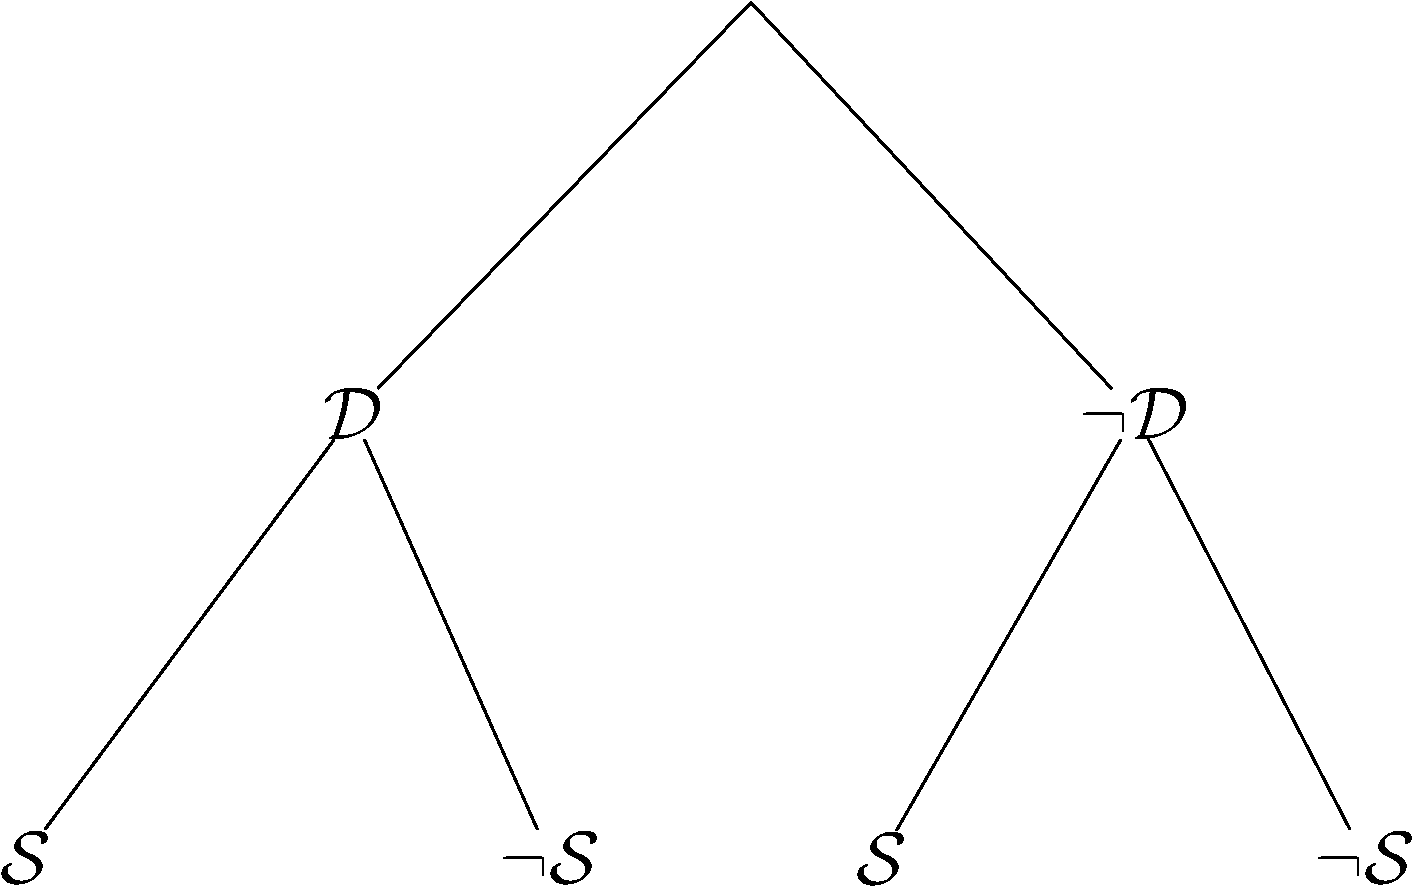
\includegraphics[width=\linewidth]{figures/treenoprobs}
\caption{A tree diagram of the events $\mathcal{D}$ (has a disease) and $\mathcal{S}$ (has a symptom).\label{fig:treenoprobs}}
\end{marginfigure}
Another way to think about marginalization is to draw a tree where you have the event, which you are marginalizing out ($\mathcal{D}$ in the previous exercise) at the first level of the tree and the variable you want to know the probability of ($\mathcal{S}$ in the previous exercise) at the next junction in the tree (see Figure~\ref{fig:treenoprobs}).


Further, we annotate the arrows with the conditional probability of the event conditioned on the things further up in the tree (note that for $\mathcal{D}$ there is nothing further up the tree, so we just write $p(\mathcal{D})$ or $p(\neg \mathcal{D})$).

\begin{center}
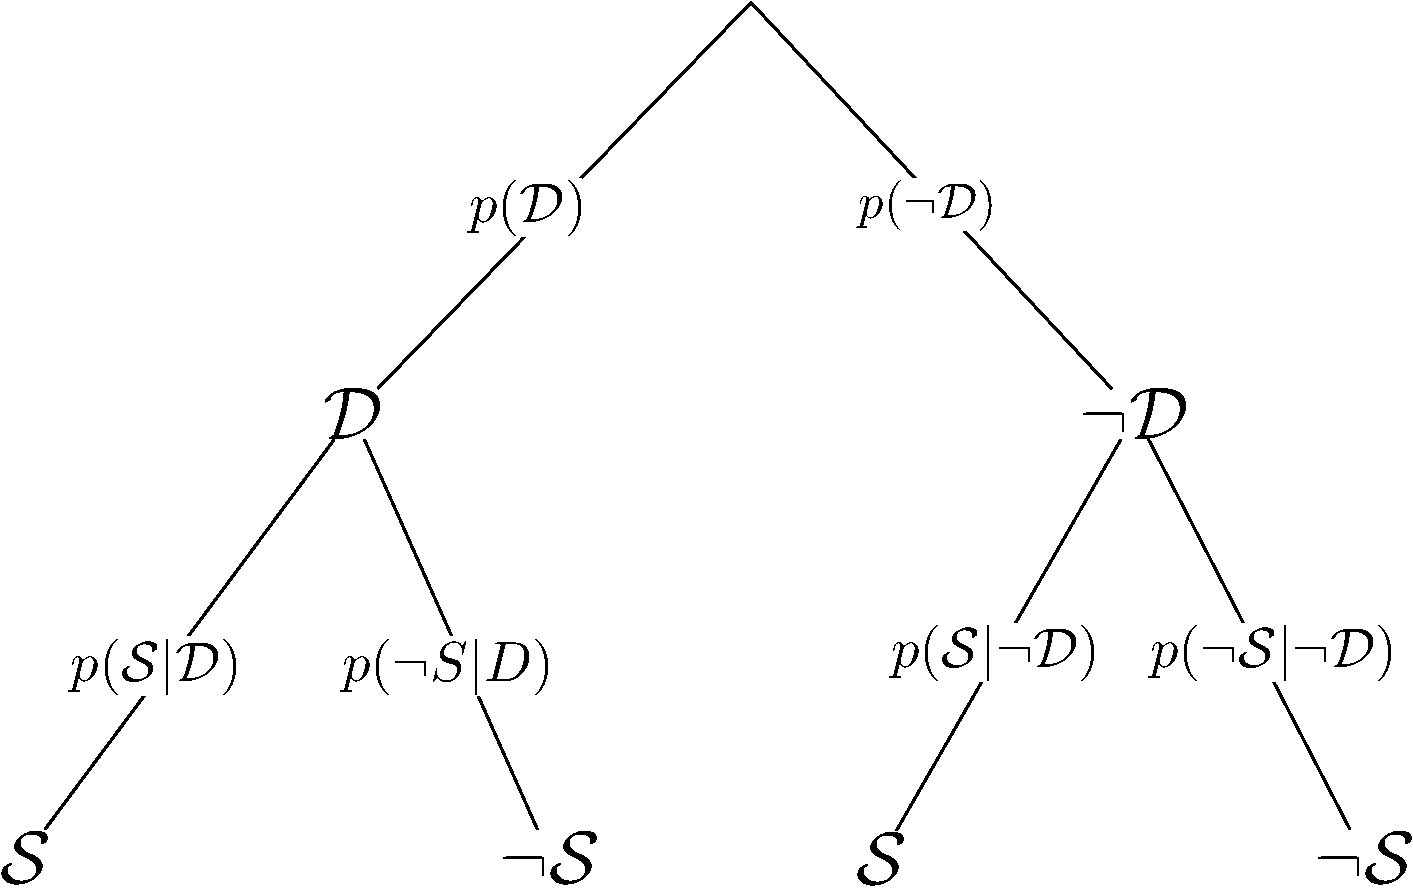
\includegraphics[width=0.6\linewidth]{figures/treeprobs}
\end{center}

If you want to find a joint probability (e.g., $p(\mathcal{D}, \neg \mathcal{S})$), follow the corresponding path, multiplying probabilities as you go.  For example, from examining the graph above we get
\begin{align}
p(\mathcal{D}, \neg \mathcal{S}) &= p(\mathcal{D}) p(\neg \mathcal{S}|\mathcal{D}) \enspace .
\end{align}

A marginal probability for an event (e.g., $p(\mathcal{S})$) can be found by summing over all paths that arrive at the event.  For example, from examining the graph above we see that there are two paths to $\mathcal{S}$, which allows us to compute $p(\mathcal{S})$ as
\begin{align}
p(\mathcal{S}) &= p(\mathcal{D}) p(\mathcal{S}|\mathcal{D}) + p(\neg \mathcal{D}) p(\mathcal{S}|\neg \mathcal{D})  \enspace .
\end{align}


\begin{exercise}[(20 minutes)]
Do problem 2 from \href{http://wwwf.imperial.ac.uk/~atw/Bayes.pdf}{this assignment}.  They use $\mathcal{E}'$ to refer to the event $\neg \mathcal{E}$.
\begin{boxedsolution}
Solution is embedded in the link.
\end{boxedsolution}
\end{exercise}

\end{document}
